
\documentclass[10pt,a4paper]{article}
\usepackage{listings}
\usepackage[usenames,dvipsnames]{color}
\usepackage{graphicx}
\usepackage{subfig}
\usepackage[margin=1in]{geometry}

\author{Sebastien Duc}
\date{\today}
\title{$1^{\mathrm{st}}$ mini project - ICA}

\begin{document}
\maketitle
\definecolor{orange}{rgb}{1,0.5,0}
\lstset{language=python,keywordstyle=\color{orange},commentstyle=\color{blue},basicstyle=\footnotesize}
\section{Single IC}
\subsection{Code}
The code is in python, it was made to work on \texttt{python 2.7}. To plot the results, the package matplotlib was used. To use the program type \texttt{python ica.py mixsquarecos}.
You can also choose which function will be used by the algorithm by typing \texttt{python ica.py mixsquarecos func} where func must be \texttt{exp}, \texttt{tanh} or \texttt{ycube}. By default \texttt{tanh} is used.

Basically there are two main python files. The first one is \texttt{fastICA.py} which contains all the functions used for the
algorithm.
\lstinputlisting[language=python,frame=single]{fastICApart1.py}
The second is \texttt{ica.py} which first mix the signals, apply fastICA on it and then plot the result.
\lstinputlisting[language=python,frame=single]{icapart1.py}
\subsection{convergence measurement}
We can say that the algorithm converges when $w$ and $w_{new}$ point in the same direction where $w_{new}$ is the new vector found by the algorithm whereas $w$ is the one from the previous step. Note that this is equivlent to say that their inner product is 1 since both are normalized.
The following line was used, where epsilon is the inner product and lim is chosen number which should be very small
\begin{lstlisting}[language=python]
abs(epsilon -1) < lim
\end{lstlisting}
\subsection{Comparison of $g$ functions}
First of all, when we run fastICA with $g(y) = y^3$, the algorithm diverges. At each step, $w_{new} = -w$.

With the other functions, namely $\tanh$ and $y\exp(-y^2/2)$, the convergence is good and fast. But there is still a difference between them. To compare them we used a loop that run the algorithm $n$ times. Each time the algorithm is ran, we compute the number of steps before convergence and we compute 
the mean over the n iterations. For the tests, we have set $\mathrm{lim} = 10^{-20}$. We conclude that $\tanh$ converges almost surely and in 5 steps in mean. For $y\exp(-y^2/2)$ the algorithm diverges sometimes but otherwise it converges quiet fast. It converges in 4 steps in mean, which is a bit faster. 
Note that to run a test, type \texttt{python ica.py convergence}.

\subsection{Results}
When using functions $\tanh$ and $y\exp(-y^2/2)$, the results are very convincing. To find the other component, we exploited the fact that the dimension is two. W simply multiplied the data with an orthogonal vector of the $w$ we got with the algorithm.
In the code the change is very simple. In the function \texttt{fastICA} of file \texttt{fastICA.py}, we just changed the return value to
\begin{lstlisting}[language=python]
return np.dot(data,w),np.dot(data,np.array([w[1],-w[0]]))
\end{lstlisting}
In Figure~\ref{fig:results1} you can see the plots of the recovered cos and square singals. Note that only the first 200 samples are plotted. 
\begin{figure}
    \centering
    \subfloat[Recovered cos]{\includegraphics[width=0.5\textwidth]{recoveredcos}}
    \subfloat[Recovered square]{\includegraphics[width=0.5\textwidth]{recoveredsquare}}
    \caption{Results of part 1}
    \label{fig:results1}
\end{figure}

\section{All ICs}
\subsection{Code}
To use the program type \texttt{python ica.py mixsouds}. As before you can also choose function g. The estimate of the signals that are output by the program are saved in directory \texttt{output}.
For this part the same python files were used. First in \texttt{fastICA.py} two functions were added. \texttt{sym\_decorrelation} and \texttt{fastICAall} which is 
as function \texttt{fastICA} but adapted to retrieve multiple sources.
\lstinputlisting[language=python,frame=single]{fastICApart2.py}
Then in file \texttt{ica.py} we added function \texttt{mixsounds\_ica} to run fast ICA on the mixed sounds. We also added lines at the end to store the results in
\texttt{.vaw} files
\lstinputlisting[language=python,frame=single]{icapart2.py}
Then to recover the initial sounds, we had to work a little more since the output of fastICA is an array of floats with wrong scale beacause of whitening step. We know that we must represent the arrray in bytes, or more simply with integers from 0 to 255.
We added the following lines at the end of function \texttt{fastICAall} to have a proper scale.

\begin{lstlisting}[language=python,frame=single]
## recover unmixed signals
# first get the estimate of the data as before 
dataest = np.array([np.dot(data,w[i]) for i in range(nIC)])
# the scale things so that it fitts between 0 and 255
dataest = dataest.T*(127)/np.max(np.abs(dataest), axis = 1)
return (dataest + 127).T
\end{lstlisting}

\subsection{Symmetric orthogonalization}
Symmetric orthogonalization is used to decorrelate the $w_i$ so that not all of them converge to the same maximum value. This allows us to retrieve all the signals that are mixed.
\subsection{Results}
For the mixed square and cos, the algorithm was applied. You can see the plots in Figure~\ref{fig:res3}.
\begin{figure}
    \centering
    \subfloat[Recovered cos]{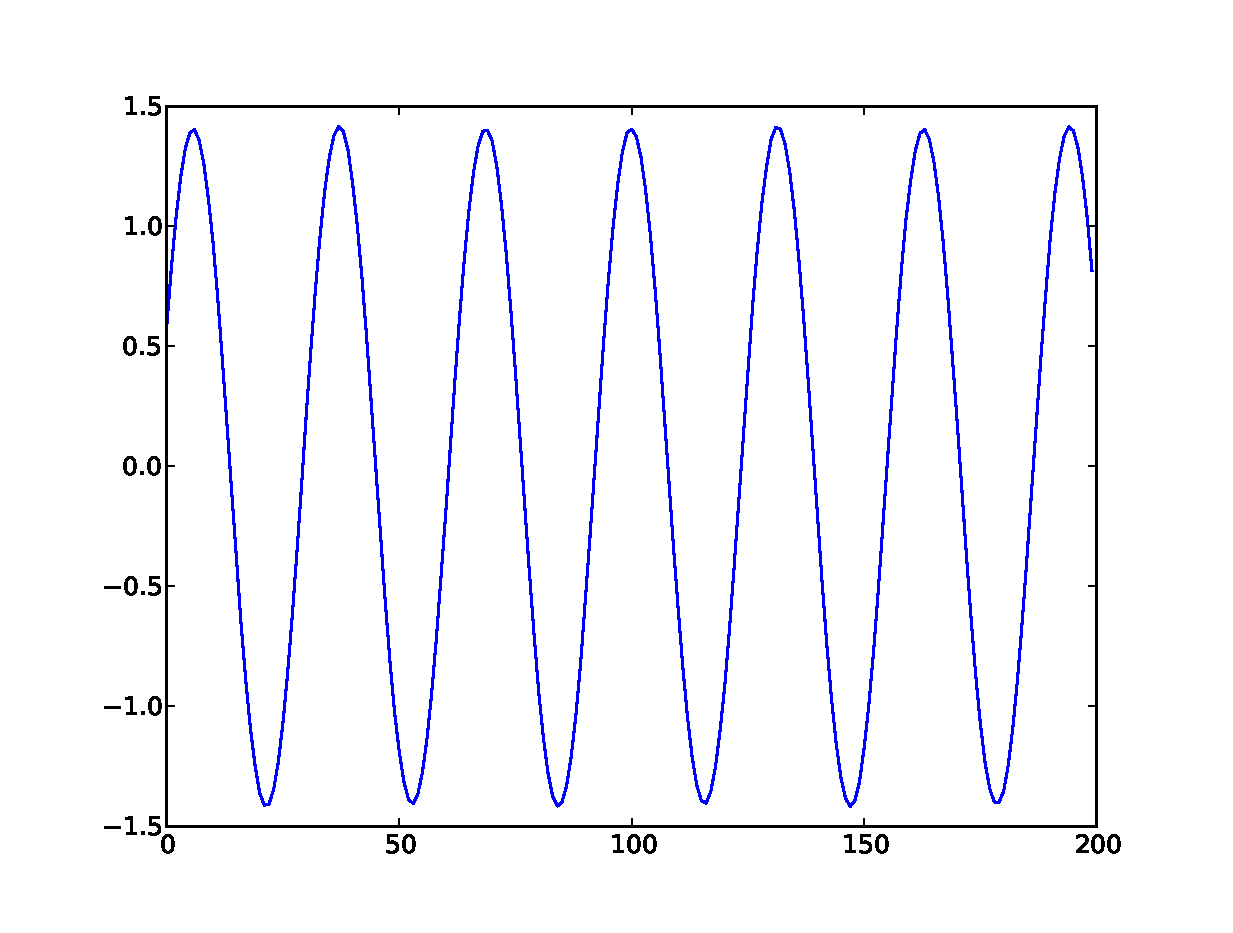
\includegraphics[width=0.3\textwidth]{recoveredcosall}}
    \subfloat[Recovered square]{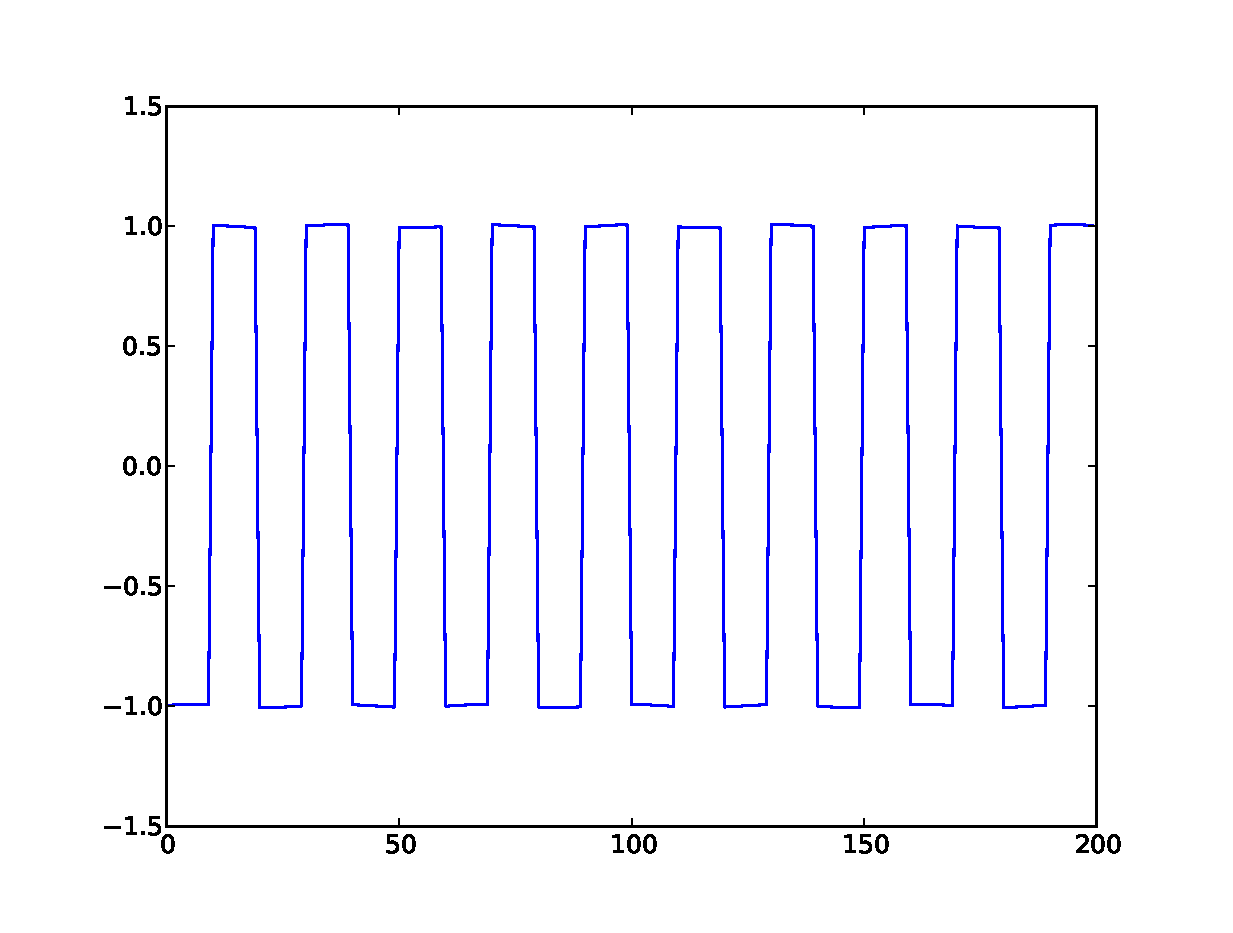
\includegraphics[width=0.3\textwidth]{recoveredsquareall}}
    \caption{Plots when applying the algorithm to recover all components on mixsquarecos}
    \label{fig:res3}
\end{figure}
For the sounds, when using fastICA we get the following plots depicted in Figure~\ref{fig:results2}. They are pretty close to the original sound but they are centered and whitened, thus don't have the same amplitude. Some of them are also sign reversed which is due to our convergence criterion because of its absolute
value.
\begin{figure}
    \subfloat[Recovered sound 1]{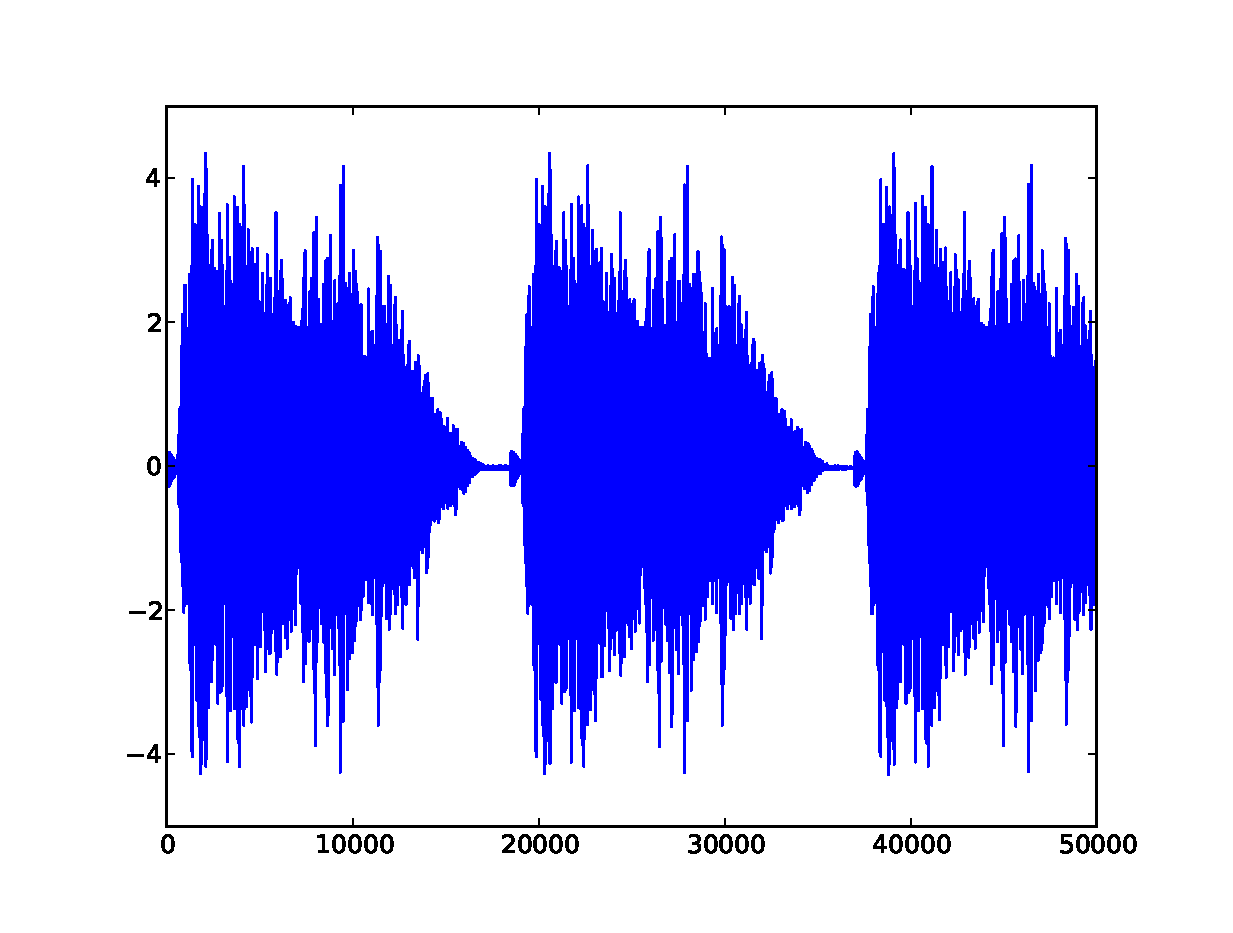
\includegraphics[width=0.3\textwidth]{recoveredsound1}}
    \subfloat[Recovered sound 2]{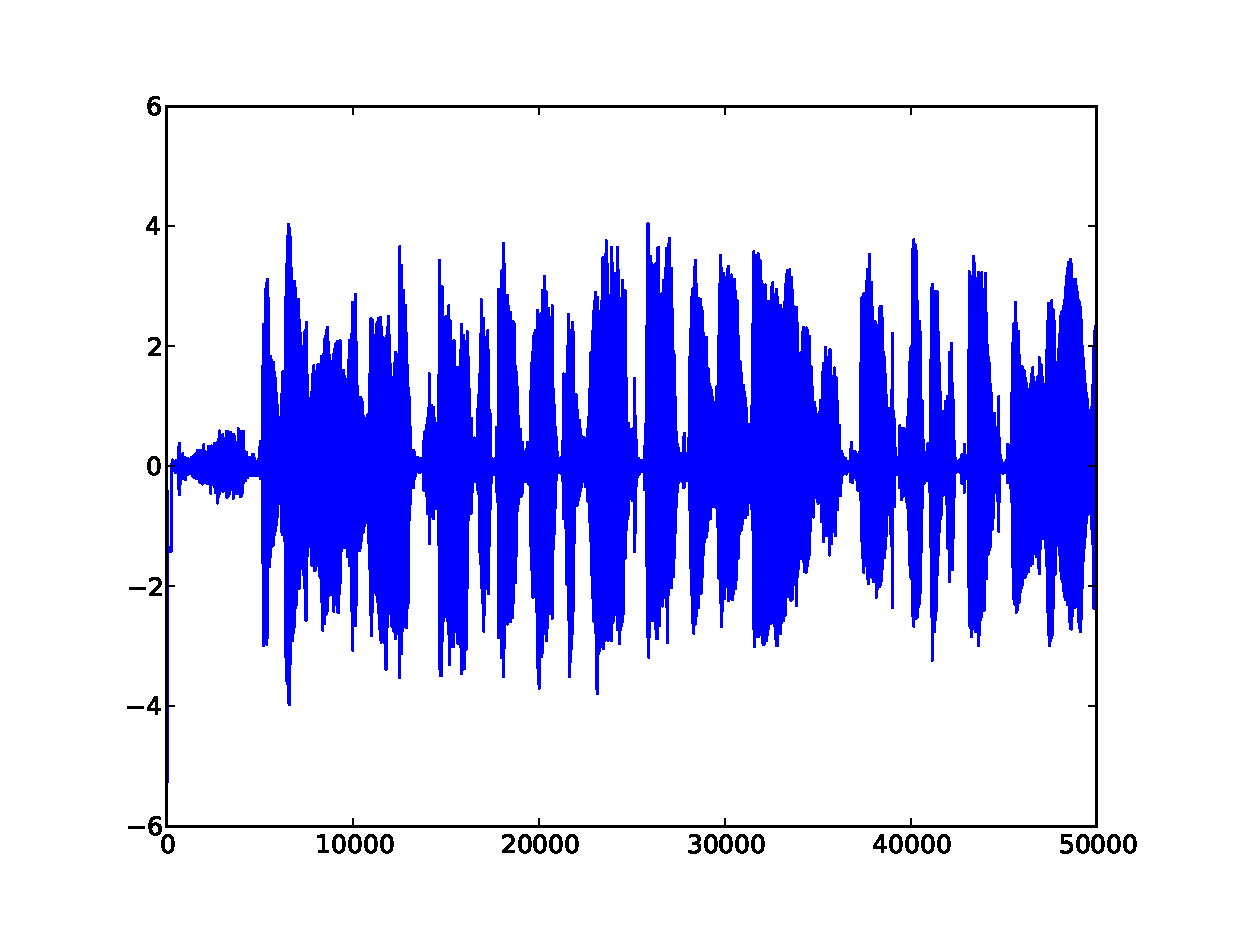
\includegraphics[width=0.3\textwidth]{recoveredsound2}}
    \subfloat[Recovered sound 3]{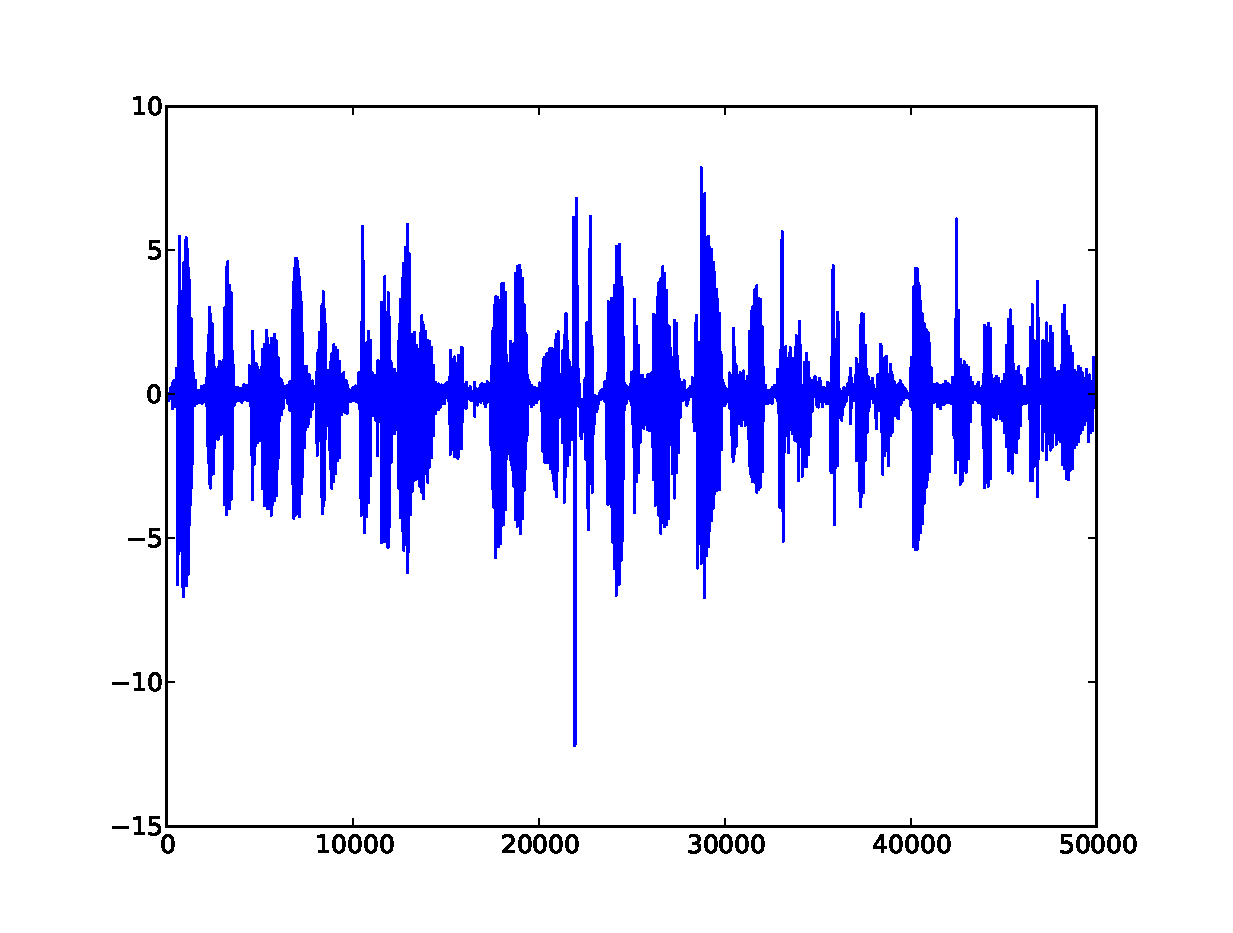
\includegraphics[width=0.3\textwidth]{recoveredsound3}}\\
    \subfloat[Recovered sound 4]{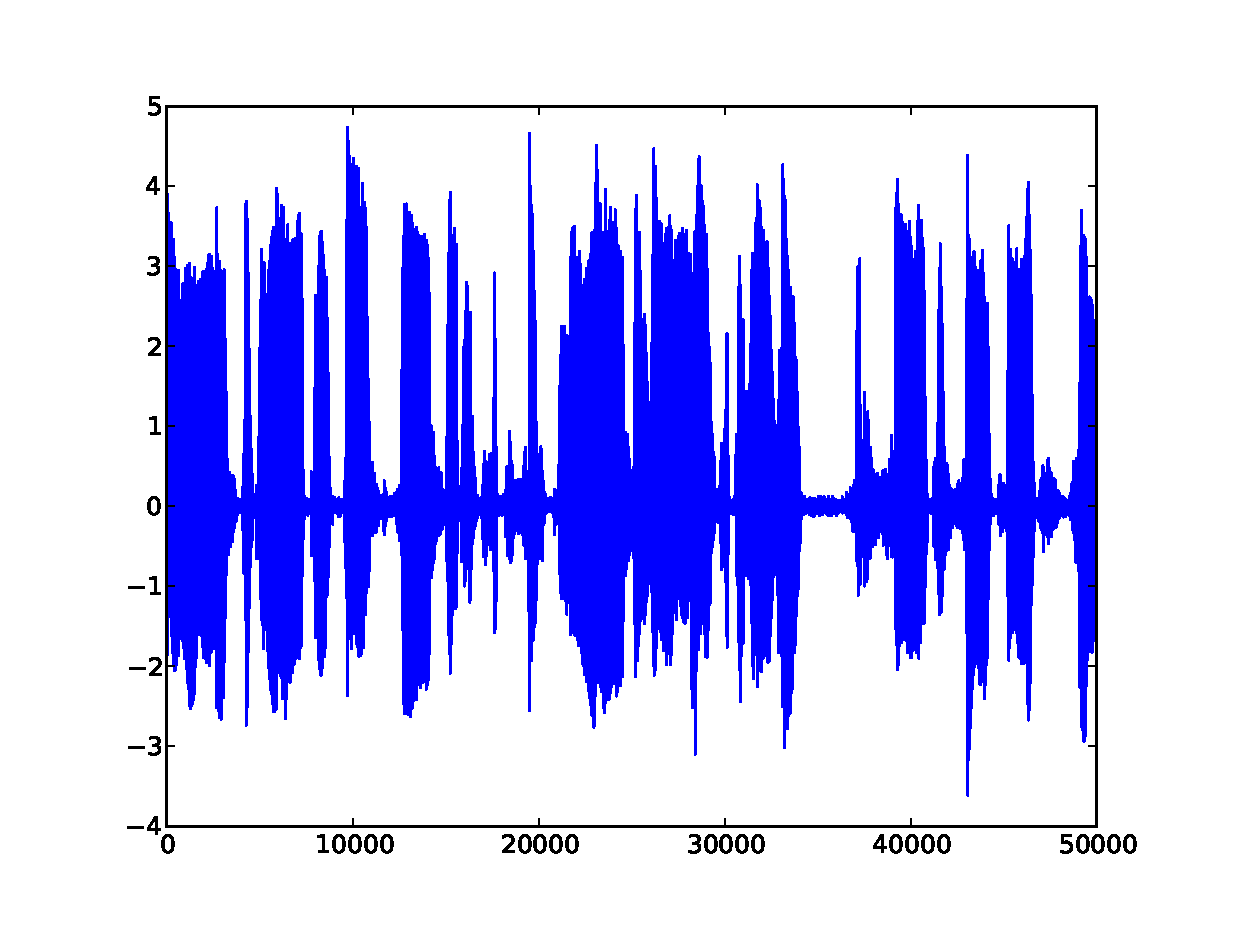
\includegraphics[width=0.3\textwidth]{recoveredsound4}}
    \subfloat[Recovered sound 5]{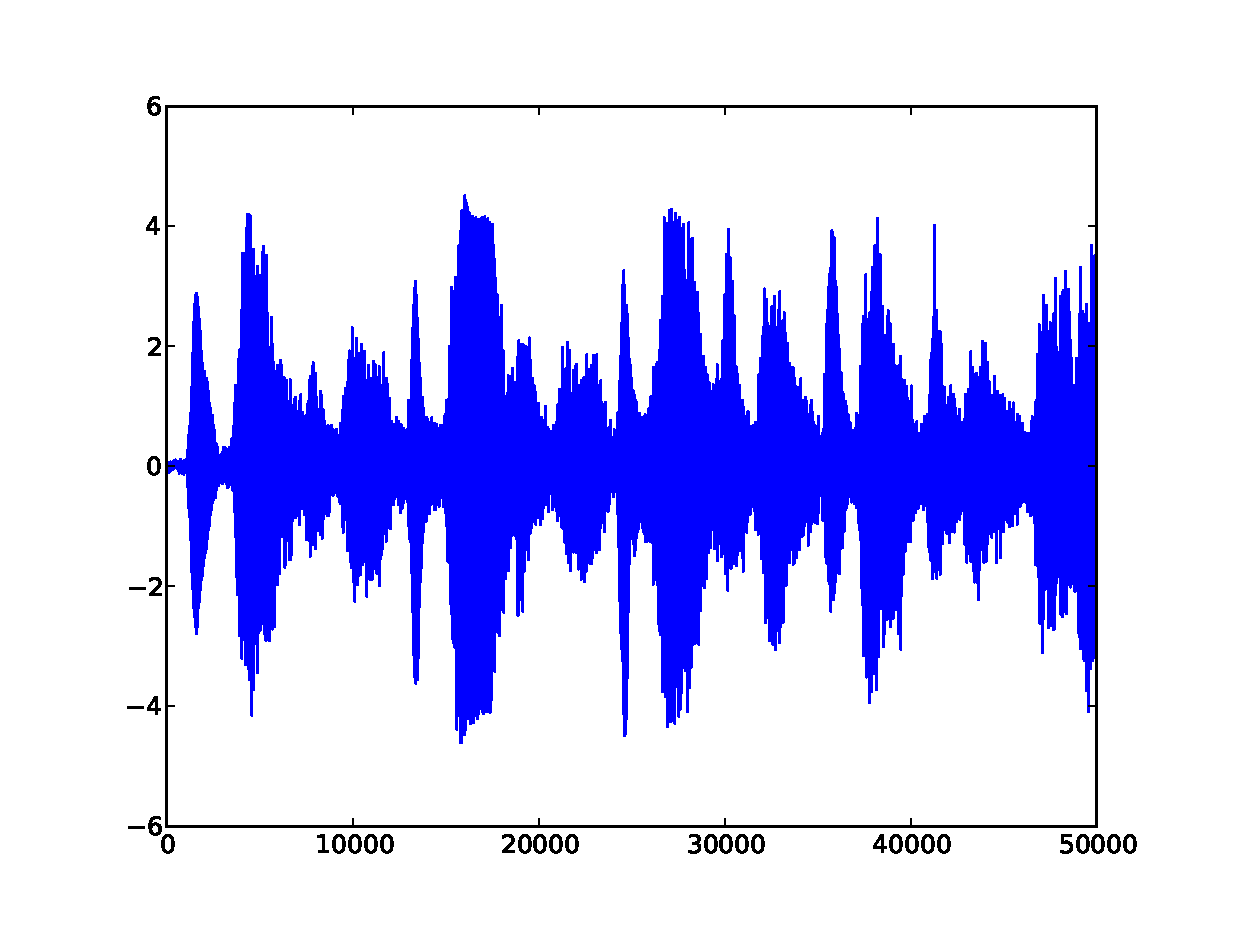
\includegraphics[width=0.3\textwidth]{recoveredsound5}}
    \subfloat[Recovered sound 6]{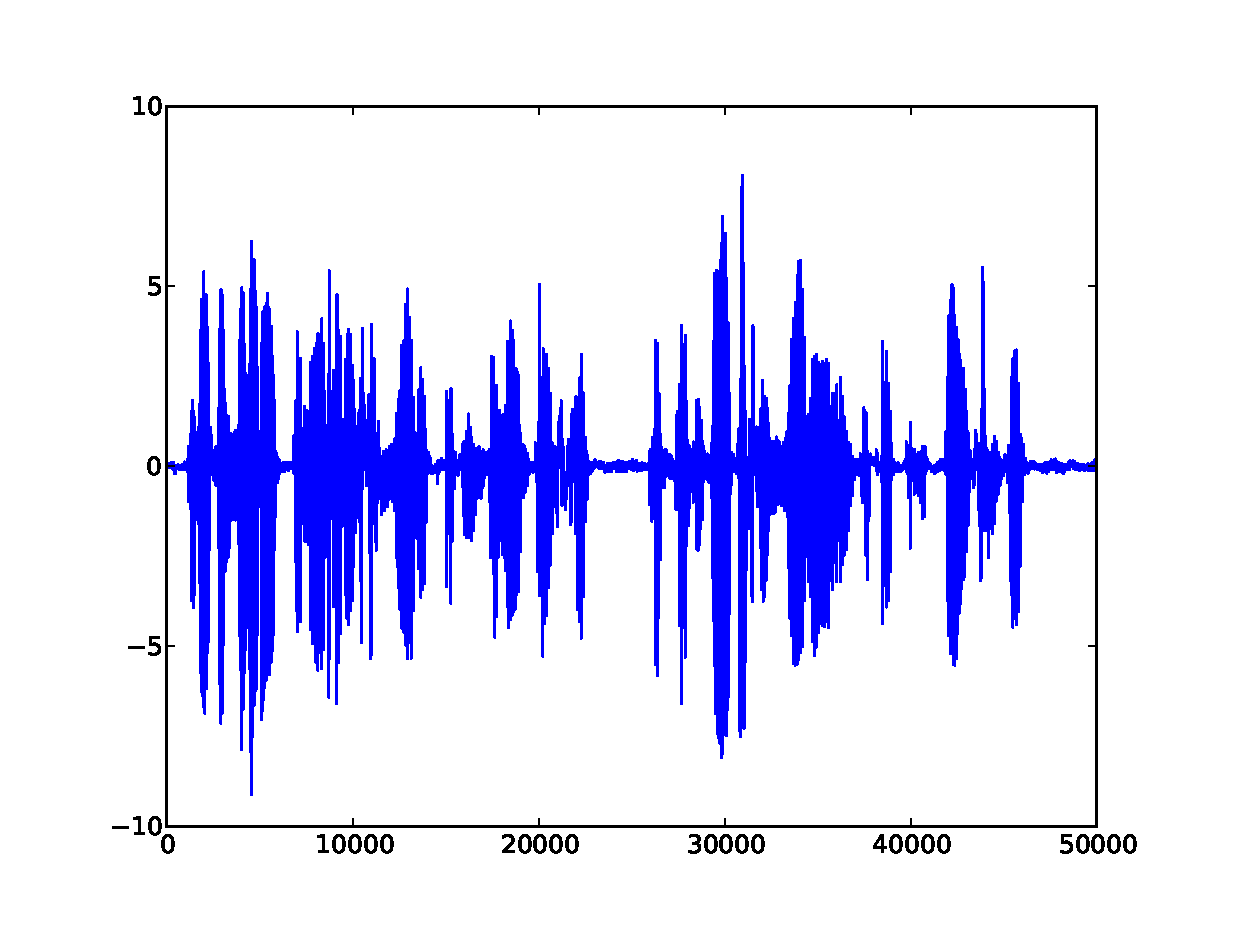
\includegraphics[width=0.3\textwidth]{recoveredsound6}}\\
    \subfloat[Recovered sound 7]{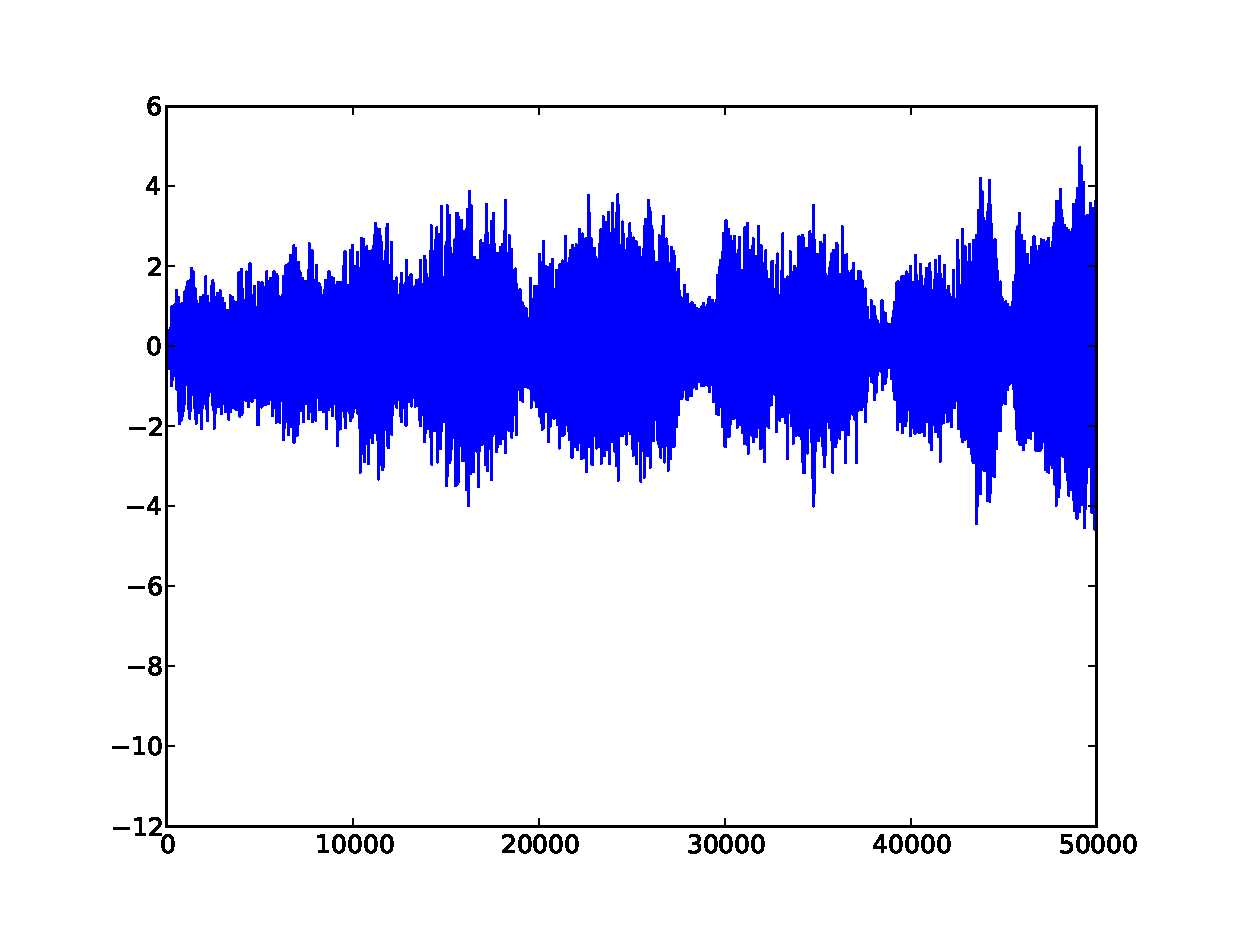
\includegraphics[width=0.3\textwidth]{recoveredsound7}}
    \subfloat[Recovered sound 8]{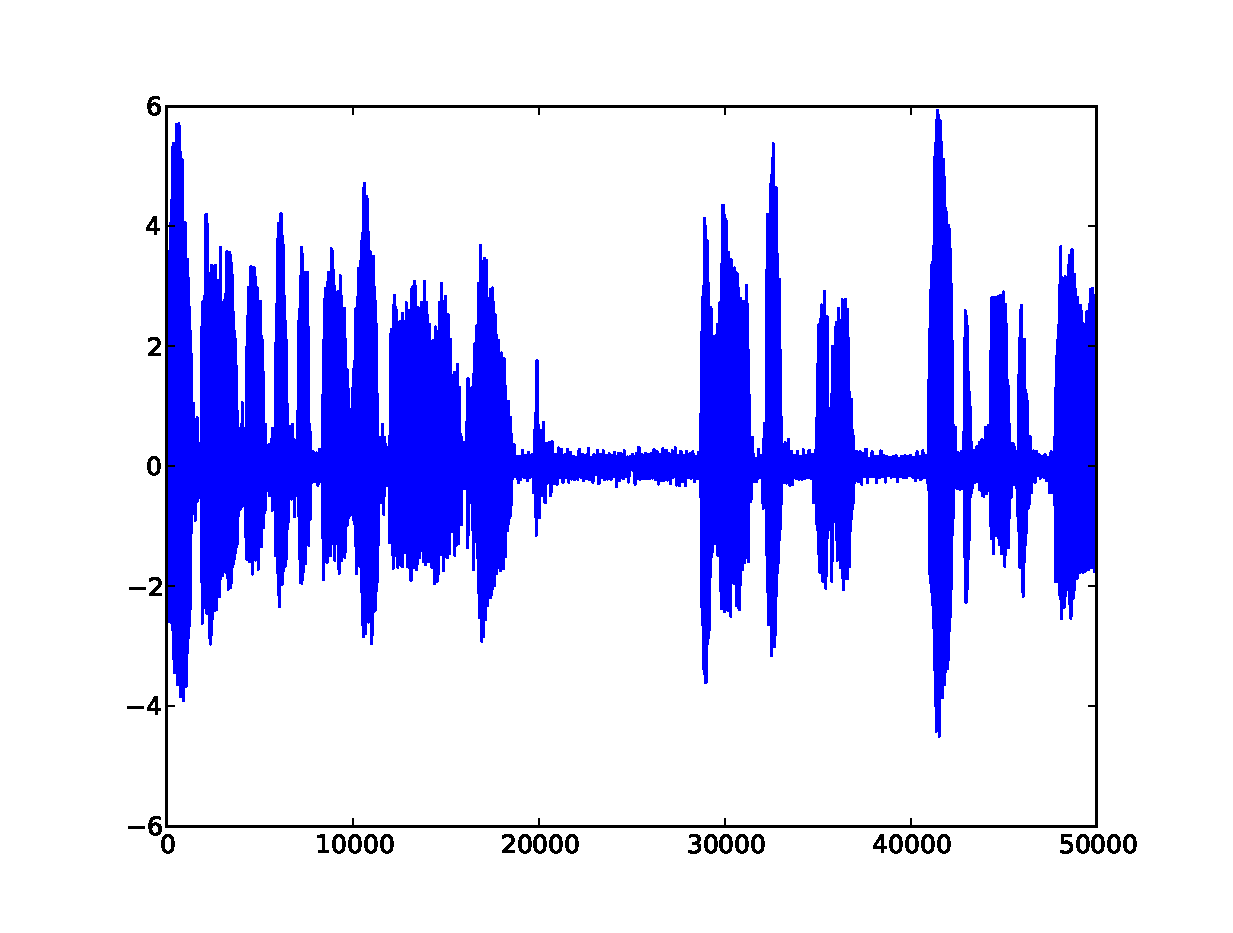
\includegraphics[width=0.3\textwidth]{recoveredsound8}}
    \subfloat[Recovered sound 9]{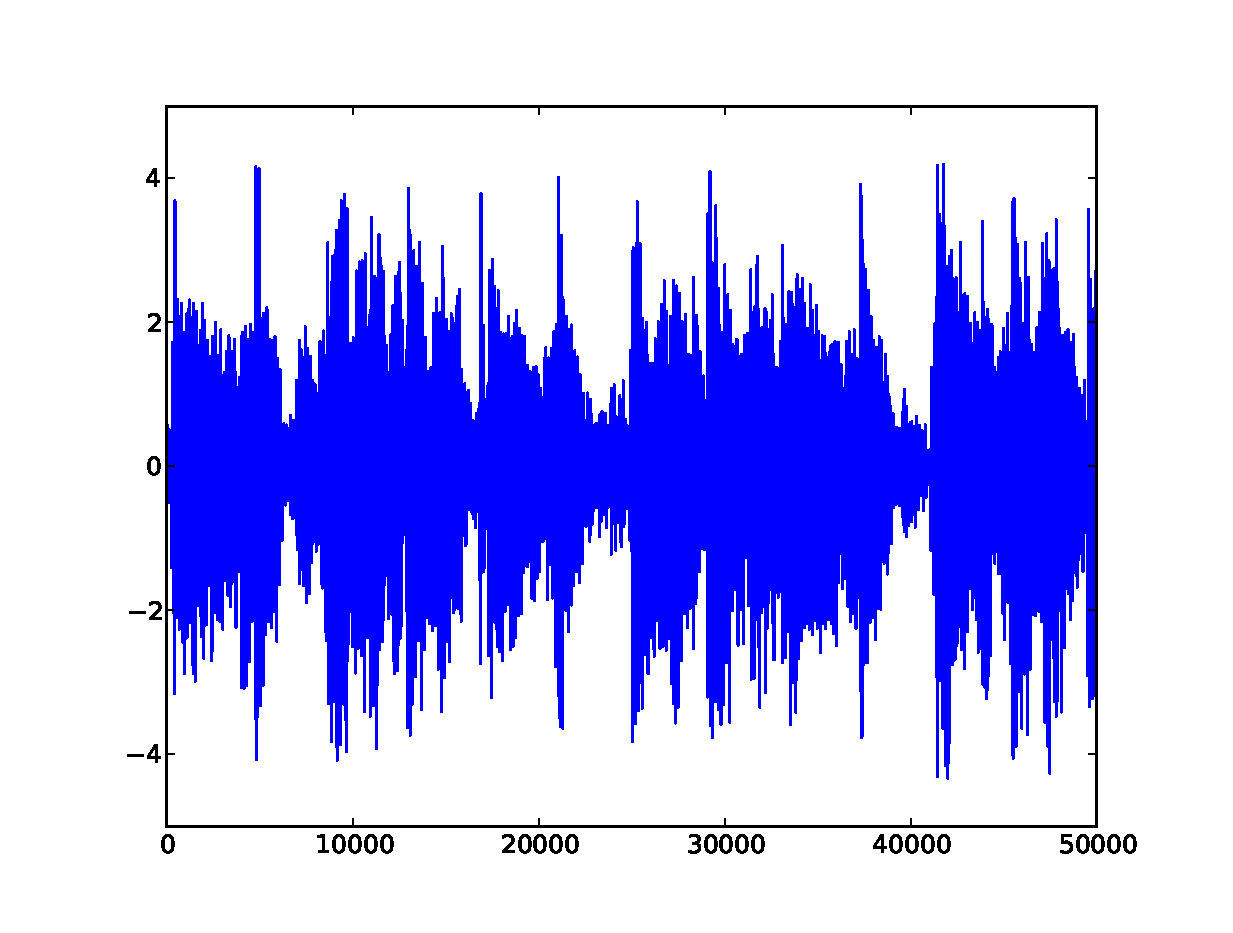
\includegraphics[width=0.3\textwidth]{recoveredsound9}}
    \caption{Results of part 2}
    \label{fig:results2}
\end{figure}

\end{document}
